\documentclass[11pt]{article}

% Encoding
\usepackage[utf8]{inputenc}
\usepackage[T1]{fontenc}

% Professional preprint style (adopted from the User-as-Code arXiv template).
\usepackage{arxiv}

% Content packages
\usepackage{amsmath}
\usepackage{amssymb}
\usepackage{graphicx}
\usepackage{array}
\usepackage{booktabs}
\usepackage{listings}
\usepackage{subcaption}
\usepackage{enumitem}
\usepackage{natbib}
\usepackage{xcolor}
\usepackage{algorithm}
\usepackage{algpseudocode}

\usepackage{microtype}
\usepackage{hyperref}
\usepackage{url}
\hypersetup{
  colorlinks=true,
  linkcolor=arxivaccent,
  citecolor=arxivaccent,
  urlcolor=arxivaccent,
  filecolor=arxivaccent,
  breaklinks=true,
}

% --- listing styles (carried over from the template) ---
\definecolor{codebg}{rgb}{0.95,0.95,0.97}
\definecolor{codegreen}{rgb}{0.0,0.5,0.0}
\definecolor{codegray}{rgb}{0.5,0.5,0.5}
\definecolor{codepurple}{rgb}{0.58,0,0.82}
\definecolor{codeblue}{rgb}{0.0,0.0,0.7}
\definecolor{alertbg}{rgb}{1.00,0.96,0.94}
\definecolor{alertred}{rgb}{0.70,0.10,0.10}

\lstdefinestyle{cstyle}{
    backgroundcolor=\color{codebg},
    basicstyle=\ttfamily\small,
    breaklines=true,
    captionpos=b,
    commentstyle=\color{codegreen},
    keywordstyle=\color{codeblue}\bfseries,
    numberstyle=\tiny\color{codegray},
    stringstyle=\color{codepurple},
    showstringspaces=false,
    numbers=left, numbersep=5pt, frame=single, rulecolor=\color{codegray}, tabsize=4,
}
\lstdefinestyle{shellstyle}{
    backgroundcolor=\color{codebg},
    basicstyle=\ttfamily\footnotesize,
    breaklines=true, language={}, showstringspaces=false,
    numbers=none, frame=single, rulecolor=\color{codegray}, tabsize=2,
}
\lstset{style=cstyle}

% --- float placement: let pages pack more floats and leave fewer gaps ---
\renewcommand{\topfraction}{0.92}
\renewcommand{\bottomfraction}{0.85}
\renewcommand{\textfraction}{0.06}
\renewcommand{\floatpagefraction}{0.72}
\setcounter{topnumber}{3}
\setcounter{bottomnumber}{2}
\setcounter{totalnumber}{5}

\title{OneBarrier: What a Network Must Provide for\\Transparent Fault Tolerance to Be Free}

\author{
  Bojie Li \\
  Pine AI
}

\date{}
\runningtitle{OneBarrier: Transparent Fault Tolerance over a Total-Order Network}

\begin{document}
\maketitle

\begin{abstract}
Transparent fault tolerance---making an unmodified server binary survive crashes, with no
code changes---has been pursued for four decades and has never reached production. Every
attempt paid three costs on the critical path of every request: recording the order in
which messages arrive, so a failed replica can be replayed; coordinating a globally
consistent snapshot; and holding each reply until the state that produced it is durable.
Industry chose instead to rewrite applications for frameworks that are fault-tolerant by
construction, leaving the installed base of stock servers behind.

This paper argues that the three costs are not intrinsic to fault tolerance: they are the
price of running over a network that guarantees neither order nor delivery. We state four
explicit conditions under which all three vanish. Three concern the network: messages are
delivered in a single global order (O); delivery is confirmed by a commit barrier (R); and
each message is replicated to backups before its barrier completes (D). Under them, the
order log is unnecessary, a consistent snapshot needs no coordination, and the output hold
ends at a barrier the network crosses anyway, so fault tolerance adds no round trip. The
fourth condition, local determinism (L), falls to the host; we show a user-space shim
closes it for unmodified binaries at a few percent overhead by virtualizing time,
randomness, and thread scheduling.

OneBarrier realizes all four conditions, supplying O, R, and D from an in-network
total-order fabric (1Pipe) with microsecond round trips. Fifteen stock
applications---including Redis, Memcached, Nginx, Node.js, and a multi-process
PostgreSQL---recover byte-identically; recovered histories are linearizable and
exactly-once under crash injection; the core protocols are machine-checked in TLA+.
Measured head to head, a durable write placed inside the barrier adds $4.6\,\mu s$ to a
request, while the same write placed after the barrier adds three milliseconds. On a
network that meets the conditions, fault tolerance is a property, not a tax.
\end{abstract}

\begin{center}
\small
Code: \url{https://github.com/bojieli/OneBarrier}
\end{center}
\vspace{-0.2em}

\begin{center}
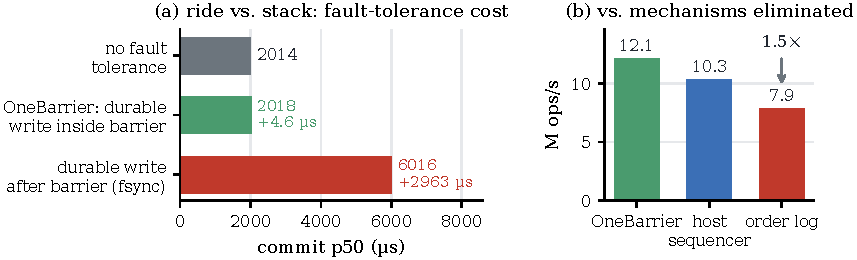
\includegraphics[width=0.98\linewidth]{figures/fig_headline.pdf}
\captionof{figure}{Headline results. (a) Ride versus stack
(\S\ref{sec:eval-overlap}): a durable write placed \emph{inside} the network's commit
barrier (condition D) adds $4.6\,\mu s$ to the p50 commit path, while the same write
placed \emph{after} the barrier adds $2963\,\mu s$---the classical output-commit cost,
reappearing exactly when condition D is broken. (b) At 8 concurrent producers,
OneBarrier outruns same-engine reimplementations of the two mechanisms the conditions
eliminate (\S\ref{sec:eval-cost}): the per-message order log ($1.5\times$) and the
host-software sequencer.}
\label{fig:headline}
\end{center}
\vspace{-0.4em}

% ===========================================================================
% OneBarrier — body.tex  (Framing C: operating-point unifier)
% ===========================================================================

\section{Introduction}

Making a server fault-tolerant without rewriting it---\emph{transparent} fault
tolerance---has been a recurring goal of systems research for four decades, and it
has repeatedly failed to reach production. The reason was never the snapshot.
Checkpointing a process is well understood. The reason was three \emph{coupled}
costs that a transparent system must pay on the critical path, and that were all a
large fraction of application latency at the operating point every prior system
lived at:
\begin{enumerate}[leftmargin=1.4em,itemsep=1pt,topsep=2pt]
\item \textbf{Logging non-determinism.} To replay a recovered replica to the exact
  state of the failed one, every non-deterministic event---above all the
  \emph{order} in which concurrent messages were processed---must be recorded.
  Order logging is the dominant per-event overhead of deterministic
  replay~\cite{castor,rr}.
\item \textbf{Coordinating a consistent cut.} A snapshot of a distributed system
  must be globally consistent; the classical mechanism is Chandy--Lamport marker
  propagation~\cite{chandylamport}, which captures in-flight channel state.
\item \textbf{Output commit.} Output that has become externally visible cannot be
  un-sent on recovery, so a transparent system must \emph{withhold} each
  externalizing message until the state that produced it is durable
  \cite{stromyemini}. This output-hold is what sank Remus~\cite{remus}: tens of
  milliseconds of latency added to every client reply.
\end{enumerate}

Faced with these costs, the industry chose the \emph{other} path: rewrite
applications so that state is externalized into a system that is fault-tolerant by
construction---durable execution (Temporal, DBOS, Restate~\cite{temporal}) and
exactly-once stream processing (Flink~\cite{flink}). That path won mindshare, but
it won it one rewrite at a time. The legacy fleet---millions of lines of stock
Redis, Memcached, Nginx, application servers, and databases---was left behind,
because rewriting them is exactly the cost transparent FT was meant to avoid.

\paragraph{This paper.} We revisit the abandoned transparent path and show that it
becomes practical under two co-designed shifts, neither sufficient alone.

The \textbf{first} shift is a user-space \emph{determinism libOS}: an
\texttt{LD\_PRELOAD} shim, with no kernel and no application changes, that makes an
unmodified server deterministically recoverable by virtualizing its residual
\emph{local} non-determinism---reads of the clock, of the random source, and the
order of thread scheduling. We show that for real servers the residual local
non-determinism, once the message order is supplied externally, is small and
closable: stock Redis, Memcached, Nginx, Node.js, and a multi-process PostgreSQL
all recover \emph{byte-identically} across a crash and a real-time gap, at a
few-percent steady-state overhead.

The \textbf{second} shift is the operating point. Prior transparent systems paid
the three costs over software-ordered, TCP-scale, hypervisor-logged
\emph{millisecond} paths, where each was a large fraction of request latency. If
instead all inter-process communication of \emph{share-nothing} servers is routed
through an in-network total-order \emph{reliable} fabric---1Pipe~\cite{onepipe},
which establishes total order in a programmable switch and delivers reliably with a
two-phase commit barrier at $1$--$2\,\mu s$ RTT---then the three costs do not merely
shrink; they \emph{change structure}:
\begin{itemize}[leftmargin=1.4em,itemsep=1pt,topsep=2pt]
\item the fabric \emph{is} the order, so the replay order-log vanishes;
\item a timestamp-$T$ snapshot replaces the Chandy--Lamport cut---and is in fact
  stronger, because an order-preserving fabric has no in-flight channel state to
  capture; and
\item the output-commit barrier \emph{coincides} with the fabric's reliable-delivery
  commit barrier, so the durable-replica write rides under a barrier the system
  already pays for, and fault tolerance adds $\approx 0$ latency over the
  reliable-fabric baseline.
\end{itemize}
The single new engineering idea is the last point: fold the durable-replica write
into phase~1 of 1Pipe's two-phase commit so that the phase-2 delivery
acknowledgement doubles as the durability acknowledgement. At the millisecond
scale this overlap saves little; at $1$--$2\,\mu s$ RTT it is the difference between
fault tolerance being a tax on every reply and being a byproduct of the
communication fabric.

\paragraph{Honesty about scope, stated up front.} This is a
realization-and-mea\-surement result, not a new primitive, and we are explicit about
three boundaries. (i) The conceptual idea is substantially anticipated:
LLFT~\cite{llft} already did transparent, order-log-free FT of unmodified socket
applications using totally-ordered virtual time, and HyCoR~\cite{hycor} already did
checkpoint-replay of unmodified containers. Our contribution is the co-design with
an \emph{in-network} fabric and the demonstration that the cost \emph{regime}
changes at the microsecond operating point; \S\ref{sec:novelty} states the prior
art and what survives, candidly. (ii) We do not have an RDMA testbed. The libOS,
the determinism, the recovery, the correctness checks, and the resource costs are
all \emph{real}, measured on stock binaries; the RDMA \emph{latency} of the
fabric is reproduced in a discrete-event model at the paper's published operating
point and corroborated by real RDMA verbs over software RoCE
(\S\ref{sec:eval-overlap}). (iii) The durability guarantee is in-memory $f$-of-$k$
fail-stop tolerance via in-fabric replication, not crash-consistent persistence
across correlated power loss---the FaRM/RAMCloud tradeoff~\cite{farm}.

\paragraph{Contributions.}
\begin{itemize}[leftmargin=1.4em,itemsep=1pt,topsep=2pt]
\item A transparent determinism libOS that closes the local-non-determinism
  boundary for real unmodified servers---time via a virtual clock, randomness via
  syscall-level interception, and threads via share-nothing sharding---and
  recovers stock Redis, Memcached, Nginx, Node.js, and PostgreSQL byte-identically
  (\S\ref{sec:libos}, \S\ref{sec:eval-recovery}).
\item The observation, and its quantification, that routing unmodified
  share-nothing servers through an in-network total-order reliable fabric makes the
  three coupled costs of transparent FT collapse, with the output-commit write
  folded into the fabric's commit barrier (\S\ref{sec:overview},
  \S\ref{sec:eval-overlap}).
\item An end-to-end evaluation: byte-identical recovery and state reconstruction;
  linearizability and exactly-once under injected crashes; recovery latency that is
  linear in log length and bounded by checkpointing (including CRIU of a
  multi-process database); steady-state overhead; and head-to-head resource costs
  against LLFT, HyCoR, Remus, and CRIU (\S\ref{sec:eval}).
\item Machine-checked TLA+ specifications of 1Pipe total order and of OneBarrier's
  exactly-once recovery, and a candid novelty reckoning (\S\ref{sec:impl},
  \S\ref{sec:novelty}).
\end{itemize}

\section{Why Transparent FT Failed, and What Changed}
\label{sec:why}

\paragraph{The three coupled costs.} A transparent FT system must, on every
externalizing message, guarantee that the producing state is recoverable. Three
mechanisms make that guarantee, and historically each was expensive.
\emph{Deterministic replay} reconstructs a failed replica's state by re-executing
its inputs in the same order; the order itself is non-deterministic and must be
logged, and message-order logging dominates replay overhead~\cite{castor}. A
\emph{consistent distributed snapshot} is needed so that a recovered replica
resumes from a globally coherent point; Chandy--Lamport~\cite{chandylamport}
achieves this by injecting markers and recording channel state. And
\emph{output commit}~\cite{stromyemini} forbids releasing output until its
producing state is durable, because external observers cannot be rolled back. Remus
\cite{remus} paid this last cost as tens of milliseconds of buffered output per
externalizing message; VMware FT~\cite{vmwareft} paid the order cost as
lock-step execution. At the millisecond scale, all three were a large fraction of
request latency---which is why transparent FT, despite four decades of work, never
displaced application-level replication.

\paragraph{The 1Pipe fabric.} 1Pipe~\cite{onepipe} provides \emph{scalable total
order} communication in a datacenter: messages carry timestamps, an in-network
(P4 programmable switch) min-reduce establishes a global order, and a FIFO gate at
each receiver delivers in timestamp order. Reliable delivery is a two-phase commit:
phase~1 scatters and durably stages, phase~2 commits once the barrier is agreed.
At 1Pipe's operating point---RDMA RTT $1$--$2\,\mu s$, best-effort delivery
$\sim\!10\,\mu s$, reliable delivery $+2$--$10\,\mu s$, recovery $50$--$500\,\mu s$,
and 1-RTT in-fabric RDMA replication---the per-message ordering and reliable-commit
costs are tens of microseconds, set by the fabric, not by software.

\paragraph{The operating-point argument.} Our central claim is not that the idea is
new but that the \emph{cost regime} is. The three costs that doomed transparent FT
were properties of a software-ordered, TCP-scale, millisecond world. Move to a
world where order is established in the switch and durable replication completes in
one RTT under a barrier the communication layer already crosses, and the costs stop
being mechanisms added on the FT critical path and become byproducts of a fabric
deployed for communication-correctness reasons. This is a design conclusion, not a
hardware speedup: the hardware changes \emph{which cost dominates}, and the result
---transparent passive FT at $\approx$ the reliable-fabric baseline---is the
non-obvious consequence.

\section{Overview: Fault Tolerance as a Byproduct of the Fabric}
\label{sec:overview}

Figure~\ref{fig:arch} shows the architecture. An unmodified share-nothing server
runs over the determinism libOS, which intercepts its POSIX surface: sockets are
routed to the 1Pipe fabric, and local non-determinism (time, randomness, thread
order) is virtualized so that, given the same input sequence, the server's
execution is a deterministic function of that sequence. The fabric supplies the
input order and a reliable-delivery commit barrier; an in-fabric RDMA replica
supplies durability as phase~1 of that barrier.

\begin{figure}[t]
\centering
\begin{lstlisting}[style=shellstyle]
  unmodified app  (Redis / Memcached / Nginx / Node / PostgreSQL)
       |  POSIX syscalls (sockets, time, rng, threads)
  +----v---------------------------------------------------+
  |  OneBarrier determinism libOS  (LD_PRELOAD, no kernel) |
  |   * POSIX socket   -> 1Pipe ReliableHost send/poll     |
  |   * virtual clock  (time)   * rng trap (getrandom/urnd)|
  |   * share-nothing shard     * det. replay + suppress   |
  |   * durable ordered log + timestamp-T snapshot         |
  +----+---------------------------------------------------+
       |  in-fabric RDMA replica  (durability = 2PC phase-1)
  +----v---------+
  | 1Pipe fabric |  total order + reliable 2PC commit barrier
  +--------------+  + decentralized recovery cut
\end{lstlisting}
\caption{OneBarrier: an unmodified server over the determinism libOS over the
1Pipe fabric. The fabric supplies order and the commit barrier; the libOS supplies
local determinism, replay, and output suppression.}
\label{fig:arch}
\end{figure}

The thesis is that the fabric pre-pays, for communication-correctness reasons, for
exactly the three things FT needs:

\paragraph{(a) Order $\Rightarrow$ no replay order-log.} Because 1Pipe delivers
messages in a global timestamp order, the recovered replica re-applies inputs in
\texttt{msg\_ts} order with no recorded order-log. The dominant cost of
deterministic replay is removed not by optimization but by relocation: the order
lives in the fabric. This is the state-machine-replication property~\cite{schneider}
realized over an in-network order source.

\paragraph{(b) Timestamp-$T$ snapshot $\Rightarrow$ empty-channel cut.} To snapshot,
the libOS quiesces at a barrier timestamp $T$: it stops dispatching inputs with
\texttt{ts}~$>T$, drains in-flight handlers for \texttt{ts}~$\le T$, and checkpoints.
Every message is, by the identical \texttt{ts}~$\le T$ predicate, on the same side
of the cut at sender and receiver, so the cut is consistent with \emph{no} marker
propagation and \emph{no} captured channel state---strictly simpler than
Chandy--Lamport, because an order-preserving fabric has no in-flight channel state.
The cut is uncoordinated: each node applies the same predicate independently.

\paragraph{(c) Output-commit $=$ commit barrier.} A server's reply is withheld until
the producing state is durable. In OneBarrier the durable-replica write is issued as
phase~1 of the fabric's two-phase reliable-delivery commit, and the phase-2 barrier
acknowledgement---which the fabric produces anyway to deliver the message
reliably---doubles as the durability acknowledgement. The output-commit hold and the
reliable-delivery barrier are the \emph{same} barrier. At $1$--$2\,\mu s$ RTT with
1-RTT replication, the durable write completes \emph{under} the $\sim\!1.5$-RTT
commit barrier, so FT's marginal latency over the reliable-fabric baseline is
$\approx 0$.

What makes (c) work in practice is (a)+(b)+the libOS: the recovered replica is a
deterministic function of the fabric-ordered input prefix up to the last durable
barrier, so ``the producing state is durable'' reduces to ``the input prefix is
replicated,'' which the fabric already does.

\section{A Transparent Determinism libOS for Unmodified Servers}
\label{sec:libos}

The fabric supplies order; the libOS must supply everything else needed for an
\emph{unmodified} binary to replay deterministically. This section is the
mechanism that makes ``transparent'' real. The libOS is three composable
\texttt{LD\_PRELOAD} libraries totalling a few hundred lines of C, in the
SocksDirect~\cite{socksdirect} kernel-bypass lineage; it requires no kernel module
and no application change.

\subsection{The determinism boundary}
Once message order is external, a server's remaining non-determinism is
\emph{local}: values it reads from the clock and the random source, and---if
multi-threaded---the order its threads interleave. We found, and the libOS closes,
a sharp boundary between two kinds of time reads. \emph{Request-driven} reads (one
per request, e.g.\ a timestamp stamped into a reply) replay correctly by sequence
position. \emph{Timer-driven} reads (a background timer firing on wall-clock, e.g.\
Redis's \texttt{serverCron}, Nginx's cached-time update, Memcached's LRU
maintainer) fire a \emph{different number of times} between record and replay,
desynchronizing any position-indexed scheme. The virtual clock closes this boundary
by making time a function of input events rather than of wall-clock or read count.

\subsection{Virtual clock: time virtualization}
The libOS intercepts the libc time surface (\texttt{gettimeofday},
\texttt{clock\_gettime}, \texttt{time}) and returns \emph{virtual} time
$t = \mathrm{base} + \mathrm{ticks}$, where \texttt{ticks} advances a fixed delta
per socket read---i.e.\ per deterministic input event. Every time read is then
\emph{count-independent}: it does not matter how many times, or from which timer,
the value is read, only how many inputs have been processed. \texttt{base} is
captured at the live run and persisted; the recovered run reconstructs the identical
virtual time for the identical input sequence. The mechanism is app-agnostic---it
catches any binary's libc time calls, and the vDSO is not an escape hatch because
\texttt{LD\_PRELOAD} overrides the exported symbols (a control counted exactly
$2\!\times\!10^6$ intercepted \texttt{gettimeofday} and \texttt{clock\_gettime}
calls). The sharpest demonstration is Nginx: the HTTP \texttt{Date} header,
formatted deep inside Nginx from its cached time, is byte-identical on the live and
recovered instances across a multi-second real-time gap.

\subsection{Randomness virtualization}
A server's randomness reaches it by paths that defeat library interposition.
glibc's \texttt{getrandom} wrapper is interceptable, but V8/Node, OpenSSL, and
\texttt{arc4random} issue the \emph{raw} \texttt{getrandom} syscall, and Redis~6
seeds its dictionary hash (SipHash) by reading \texttt{/dev/urandom} through
\texttt{fopen}, whose internal \texttt{openat}/\texttt{read} bypass the public
symbols. The libOS therefore intercepts at the syscall level: a seccomp-BPF
user-notification filter traps \texttt{getrandom} and fills the caller's buffer from
a deterministic stream seeded from a persisted seed; \texttt{/dev/urandom} is
redirected, via a private mount namespace, to a deterministic file. Two further
entropy sources must be pinned for V8's \texttt{Math.random}: address-space layout
(disabled with \texttt{setarch -R}) and the \texttt{RDRAND} CPU instruction, which
no syscall trap can catch (disabled for OpenSSL via \texttt{OPENSSL\_ia32cap}). With
the full stack, Node's \texttt{Date.now()} \emph{and} \texttt{Math.random()} are
byte-identical across recovery, and Redis's \texttt{SPOP}/\texttt{SRANDMEMBER}
outputs---which depend on the SipHash-seeded dictionary layout---recover identically
where a control with the real device differs entirely.

\subsection{Threads: deterministic scheduling vs.\ share-nothing sharding}
\label{sec:threads}
For a multi-threaded server the OS chooses the order threads enter critical
sections, so shared-state evolution is non-deterministic. We implemented a
Kendo-style~\cite{kendo} deterministic scheduler: a thread may take a top-level lock
only when its logical clock is the global minimum, making the interleaving a
function of the clocks rather than of OS timing. It is correct---a 4-thread
microbenchmark's critical-section order is identical across runs where it otherwise
varies---but it serializes critical sections and \emph{collapses throughput} on a
contended server (a 4-worker Memcached ran $>\!1000\times$ slower, spinning). The
practical answer is not deterministic scheduling but the \emph{share-nothing
sharding} model that high-performance servers already use: run $N$
\emph{single-thread} instances, each deterministic by construction (one thread, so
input order is whatever the fabric supplies and there are no data races), and scale
by processes, not threads. Because shards share nothing, they have no lock
contention: four single-thread Memcached shards reach $1.0$\,M ops/s aggregate,
exceeding one 4-worker process (821\,k ops/s), while staying deterministic. The
deterministic scheduler remains as the fallback for genuinely shared mutable state.
Single-thread servers still spawn timer-driven maintenance threads---Memcached's LRU
maintainer mutates LRU bookkeeping on a real-time schedule---which we disable so the
shard's state evolves purely from the request stream and the virtual clock.

\subsection{Process-state checkpoint and bounded recovery}
\label{sec:criu}
Replay from process start costs $O(\text{log})$; a checkpoint bounds it to the
post-checkpoint tail. Two mechanisms provide checkpoints. An application-native
snapshot (a Redis RDB) plus tail-replay works for a single process; combined with a
virtual-clock tick checkpoint, the recovered instance resumes time exactly where the
snapshot was taken. The general, any-binary mechanism is CRIU: it checkpoints the
whole process---memory, file descriptors, threads, \emph{and} the in-memory virtual
clock---so a restore needs no replay of the pre-checkpoint history. We verify CRIU
checkpoint/restore of the hardest app class, a multi-process PostgreSQL (postmaster
plus background workers, SysV and POSIX shared memory, WAL): data is byte-identical
across the crash and the restored server is live (\S\ref{sec:eval-recovery}).

\subsection{Output suppression and exactly-once}
On replay the server re-emits outputs it already sent before the crash. The libOS
suppresses these via a per-client \texttt{(client, seq)} high-water-mark: an output
whose sequence is at or below the client's last acknowledged sequence is dropped, so
each acknowledged effect is externalized exactly once across recovery.

\paragraph{Engineering realities.} Making ``unmodified'' credible required handling
the awkward edges of interposition: the \texttt{LD\_PRELOAD} early-init trap (the
dynamic loader calls \texttt{pthread\_mutex\_lock} before the shim's constructor
resolves it); glibc symbol versioning (\texttt{pthread\_cond\_wait} must be bound
to its \texttt{GLIBC\_2.3.2} version via \texttt{dlvsym}, or threaded servers hang);
and the seccomp filter that traps a syscall while the supervisor that services the
trap runs in the same process. These are not incidental---they are why prior
transparent systems that intercept at the library level miss the raw-syscall and
internal-call paths that real servers actually use.

\section{Fault Tolerance over the Fabric}
\label{sec:ft}

The engine that ties the libOS to the fabric is a deterministic-replay state
machine with a durable ordered log and timestamp-$T$ snapshots. On the live path it
applies fabric-delivered inputs in \texttt{msg\_ts} order, appends \texttt{(ts, op)}
to the durable log, and---when the commit barrier passes a snapshot timestamp
$T$---takes an uncoordinated empty-channel checkpoint (\S\ref{sec:overview}b). The
durable-replica write that makes an output committable is issued as phase~1 of the
fabric's reliable-delivery 2PC (\S\ref{sec:overview}c). On recovery, a replacement
replica loads the latest snapshot, replays the durable log suffix in timestamp order
(no order-log), and state-transfers any prefix it is missing from a surviving
replica via the fabric's decentralized recovery-cut agreement; output suppression
makes the replayed effects exactly-once. The guarantee is in-memory $f$-of-$k$
fail-stop tolerance: acknowledged writes survive up to $f$ correlated failures among
$k$ replicas, with durability supplied by in-fabric replication rather than stable
storage.

\section{Implementation}
\label{sec:impl}

The OneBarrier engine is $\sim$6\,k lines of Rust over the \texttt{ReliableHost}
fabric of an open 1Pipe reproduction, with a key/value state machine, a durable
ordered log, timestamp-$T$ snapshots, exactly-once output suppression, and crash
recovery; it ships 18 binaries (servers, benchmarks, fault injectors, checkers) and
31 passing tests. The libOS is three \texttt{LD\_PRELOAD} C libraries
(\texttt{libobpreload} for sockets/time/capture, \texttt{librngdet} for the seccomp
randomness trap, \texttt{libdetsched} for deterministic scheduling). We
machine-check the core protocols in TLA+: 1Pipe total order (TLC explored
$3.5\times10^6$ states with no order violation) and OneBarrier's exactly-once and
no-lost-acknowledged-write properties. Every result in \S\ref{sec:eval} is
reproduced by a single command recorded in the artifact.

\section{Evaluation}
\label{sec:eval}

We answer: does the fabric coincidence make FT's marginal cost
$\approx0$ (\S\ref{sec:eval-overlap})? Do real unmodified servers recover
byte-identically (\S\ref{sec:eval-recovery})? Are they correct under fault
(\S\ref{sec:eval-correct})? How fast is recovery (\S\ref{sec:eval-time})? What does
the libOS cost (\S\ref{sec:eval-overhead})? And how does the resource cost compare to
prior transparent systems (\S\ref{sec:eval-compete})? We lead with the parts that are
measured on real binaries.

\subsection{FT marginal cost \texorpdfstring{$\approx 0$}{~0}}
\label{sec:eval-overlap}
The make-or-break measurement isolates the marginal durability cost of FT under two
durability tiers. Table~\ref{tab:rq2} reports the in-fabric/in-memory tier (the
durable write rides the commit barrier) against serial fsync-to-storage. Absolute
microseconds are the reproduction's loopback-UDP fabric, \emph{not} RDMA; the
\emph{shape}---overlap vs.\ stack---is what transfers to the operating point.

\begin{table}[t]\centering\small
\begin{tabular}{lrrr}
\toprule
tier & delivery p50 & marginal durable p50 & commit p50 \\
\midrule
in-fabric (rides barrier) & $2014\,\mu s$ & \textbf{$4.59\,\mu s$} & $2018\,\mu s$ \\
fsync (serial storage)    & $3042\,\mu s$ & \textbf{$2963\,\mu s$} & $6016\,\mu s$ \\
\bottomrule
\end{tabular}
\caption{RQ2. With in-fabric durability the marginal FT cost is $0.23\%$ of the
delivery latency---the output-commit write overlaps the reliable-delivery barrier.
Serial fsync stacks $\sim$3\,ms on the critical path (commit doubles) and collapses
throughput. The contrast, not the absolute $\mu s$, is the result.}
\label{tab:rq2}
\end{table}

With in-fabric durability the marginal cost is $0.23\%$ of delivery latency: output
commit and reliable delivery are the same barrier. Serial fsync stacks $\sim$3\,ms
and saturates the executor (it completed only $3426/6000$ ops at full load),
confirming that stable-storage durability is out of regime at fabric speed. A
discrete-event model at the paper's RDMA operating point reproduces the overlap, and
real RDMA verbs over software RoCE (SoftRoCE/\texttt{rdma\_rxe}) measure an
\texttt{RDMA\_WRITE} latency of $\sim\!1.5\,\mu s$---squarely in the $1$--$2\,\mu s$
operating point. We are explicit that SoftRoCE is CPU-bound and therefore cannot
exhibit the RTT-bound \emph{overlap} directly; it corroborates that the verbs path
is real and the per-operation latency is in regime, while the overlap itself is
established by the model. Closing this with real hardware is the principal item
needing an RDMA testbed.

\subsection{Byte-identical recovery of five unmodified servers}
\label{sec:eval-recovery}
We record an unmodified server under the virtual clock and randomness stack, crash
it with \texttt{kill -9}, wait a multi-second \emph{real} wall-clock gap, and replay
on a fresh instance with the same persisted base; a control instance runs without
the libOS so its real-time output must differ. Table~\ref{tab:apps} summarizes:
every app's time-dependent output is byte-identical across the gap, and the control
differs. Beyond observable outputs, full application \emph{state} reconstructs
identically: a Redis store with TTL'd keys recovers byte-identical absolute
expiries; a Node session store keyed by \texttt{Math.random()} with
\texttt{Date.now()} timestamps recovers identical session IDs and timestamps;
Memcached's LRU \emph{eviction} decisions under memory pressure recover bit-exactly;
and PostgreSQL recovers byte-identical table contents through a CRIU
checkpoint/restore of its full multi-process tree, with the restored server
accepting new writes.

\begin{table}[t]\centering\small
\begin{tabular}{lll}
\toprule
server & probe & live $=$ replay across gap \\
\midrule
Redis     & \texttt{TIME}          & byte-identical (control differs) \\
Memcached & \texttt{stats time}    & byte-identical (control differs) \\
Nginx     & \texttt{Date:} header  & byte-identical (control differs) \\
Node.js   & \texttt{Date.now/rand} & byte-identical (control differs) \\
PostgreSQL& table + CRIU restore   & byte-identical, server live \\
\bottomrule
\end{tabular}
\caption{Deterministic recovery of unmodified servers. Time/RNG-dependent output is
byte-identical across a crash and a real-time gap; a no-libOS control differs.}
\label{tab:apps}
\end{table}

\subsection{Correctness under fault}
\label{sec:eval-correct}
We apply adversarial checks to a recovered \emph{unmodified} Redis. Eight concurrent
clients drive unique-key writes and a shared register; mid-load we
\texttt{kill -9} the server and recover it by replaying the captured request stream.
Every one of $191{,}073$ acknowledged writes survived recovery with its exact value
($0$ lost, $0$ torn); in-flight operations are excluded as the honest output-commit
gap. A from-scratch Wing--Gong linearizability checker confirms the concurrent
register history (including a post-recovery read) is linearizable---a real
linearizability verdict, not an acked-set heuristic.

\subsection{Recovery time and availability}
\label{sec:eval-time}
Recovery latency is linear in log length and reconstruction is exact. Replaying an
unmodified Redis's captured request stream on a fresh instance takes $35$\,ms for
$10$k requests, $87$\,ms for $100$k, and $536$\,ms for $1$M ($\sim$95\,MB/s,
$\sim$1.9\,M req/s), with the recovered key count equal to the live count at every
size. A checkpoint bounds replay to the post-checkpoint tail: with a checkpoint
every $100$k requests, recovery is $\sim$87\,ms of replay plus a restore (CRIU
restore of a server is tens of milliseconds), i.e.\ sub-$100$\,ms downtime---versus
the seconds-to-minutes detection-and-restart of cluster failover.

\subsection{Steady-state overhead of the libOS}
\label{sec:eval-overhead}
On \texttt{redis-benchmark} and ApacheBench, time virtualization costs $\sim$2--4\%
and randomness virtualization is within noise; FT request capture costs $<\!5\%$ on
realistic Nginx load (and is, in the real design, the fabric's 1-RTT replica write
rather than a local log). The one expensive component is the deterministic
scheduler (\S\ref{sec:threads}), which is why the production path is share-nothing
single-thread shards: Memcached single-thread under the full libOS sustains
$302$\,k ops/s (a $\sim$10\% FT overhead over its $342$\,k baseline), and four such
shards aggregate to $1.0$\,M ops/s---exceeding one 4-worker process while remaining
deterministic.

\subsection{Resource cost and competitors}
\label{sec:eval-compete}
Against in-harness models of prior systems, OneBarrier's passive design (one live
replica plus log and snapshot) uses $\sim$1$\times$ execution CPU where active SMR
uses $\sim$$N\times$, a $49$--$83\%$ saving; it carries no per-event non-determinism
log, unlike HyCoR; and against a real CRIU checkpoint competitor, log-based recovery
avoids periodic full-RSS image writes (CRIU checkpoint measured at $37$--$121$\,ms
for $30$--$300$\,MB). The snapshot-interval tradeoff is as the recovery model
predicts: a small interval triples steady apply cost but recovers in $20\,\mu s$; a
large interval minimizes steady cost but recovers $283\times$ slower
(full replay).

\section{What Is New: An Honest Reckoning}
\label{sec:novelty}

An adversarial prior-art review finds the conceptual thesis substantially
anticipated, and we state it plainly (Table~\ref{tab:prior}). LLFT~\cite{llft}
already achieved transparent, order-log-free FT of unmodified socket applications
by tagging messages with totally-ordered virtual time; HyCoR~\cite{hycor} already
did checkpoint-replay of unmodified containers; NOPaxos/Eris/Derecho
\cite{nopaxos,eris,derecho} already offloaded total order to the network for
\emph{active} SMR; and Remus/VMware-FT~\cite{remus,vmwareft} are the transparent
VM-FT systems whose output-hold latency we remove. The blunt objections are: ``it is
passive SMR and the vanishing order-log is Schneider's 36-year-old property''; ``LLFT
already did transparent no-order-log FT---you just substitute an in-network fabric
for the order source''; and ``the fabric is a network, not stable storage, so
output-commit needs a durability the fabric does not provide.''

\begin{table}[t]\centering\small
\begin{tabular}{p{0.16\linewidth}p{0.34\linewidth}p{0.40\linewidth}}
\toprule
prior & what it already did & gap OneBarrier owns \\
\midrule
LLFT & transparent FT of unmodified socket apps, no order-log, via totally-ordered
virtual time & order source is host software, not in-network; we offload it to the
switch and show the cost regime change \\
HyCoR & checkpoint-replay of unmodified containers & still logs non-determinism over
a normal network; we remove the order-log via the fabric \\
NOPaxos/Eris/Derecho & network-offloaded order for consensus/SMR & active SMR ($N$
execute); we are passive (1 live + log + snapshot) \\
Remus/VMware-FT & transparent VM-FT, output buffered until sync & the output-hold
latency we remove via the barrier coincidence \\
\bottomrule
\end{tabular}
\caption{Prior art that anticipates parts of the thesis, and the gap OneBarrier
owns.}
\label{tab:prior}
\end{table}

What survives is not a new primitive but a realization-and-measurement: OneBarrier
is the first system to show that routing unmodified share-nothing servers through a
single in-network total-order reliable fabric makes transparent passive FT cost
$\approx$ the total-order baseline---by folding the output-commit durable write into
the fabric's commit barrier---and to demonstrate the enabling determinism libOS on
five real unmodified servers including a multi-process database. The defense against
the durability objection is the in-fabric RDMA replica: durability is supplied as
phase~1 of the very barrier that delivers the message, so the coincidence is
complete for the $f$-of-$k$ fail-stop guarantee we claim. The defense against the
``just LLFT'' objection is the operating-point argument and its measurement: LLFT
and the others lived at the millisecond scale where the technique's overhead was a
large fraction of latency; the contribution is showing that at the microsecond,
in-network-order operating point the cost \emph{structure} collapses and a
long-dismissed technique becomes practical.

\section{Limitations and Scope}
\label{sec:limits}

We do not have an RDMA/P4 testbed: the fabric's RDMA \emph{latency} is reproduced in
a model at the published operating point and corroborated by CPU-bound SoftRoCE
verbs, so the overlap is established by the model rather than measured on hardware---
the one result that an RDMA testbed would strengthen. Durability is in-memory
$f$-of-$k$ fail-stop tolerance via in-fabric replication, not crash-consistent
persistence across correlated power loss (the FaRM/RAMCloud tradeoff~\cite{farm});
the out-of-regime fsync/cross-AZ design point stacks durability on the critical path
and is not our target. The transparent guarantee is for \emph{share-nothing}
servers; arbitrary shared-everything multithreading is the deterministic-multi\-thread\-ing
frontier, where our share-nothing sharding answer trades shared-memory scaling for
determinism. Finally, transparent FT cannot recover external side effects already
delivered to non-cooperating peers; output commit bounds, but does not eliminate,
the externally-visible inconsistency window.

\section{Related Work}
\label{sec:related}

\textbf{Transparent fault tolerance.} Remus~\cite{remus} and VMware FT
\cite{vmwareft} replicate whole VMs with buffered output and lock-step;
COLO and LLFT~\cite{llft} reduce the cost via output comparison and virtual-time
ordering; HyCoR~\cite{hycor} uses checkpoint-replay for unmodified containers.
OneBarrier shares their transparency goal and differs in routing order and
durability through an in-network fabric. \textbf{Deterministic replay.}
rr~\cite{rr} and Castor~\cite{castor} record non-determinism for replay debugging
and FT; we remove the order-log by relocating order to the fabric and virtualize the
residual local non-determinism for unmodified servers.
\textbf{Network-offloaded ordering.} NOPaxos~\cite{nopaxos}, Eris~\cite{eris}, and
Derecho~\cite{derecho} offload order to the network for consensus and active SMR;
1Pipe~\cite{onepipe} provides scalable total-order communication, which we use as a
passive-FT substrate. \textbf{Durable execution and stream processing.}
Temporal/DBOS/Restate~\cite{temporal} and Flink~\cite{flink} achieve fault tolerance
by rewriting applications to externalize state; we target the unmodified fleet that
path leaves behind. \textbf{Checkpoint/restore and deterministic multithreading.}
CRIU~\cite{criu} provides general process checkpoint, which we use for bounded
recovery; Kendo~\cite{kendo} and Dthreads~\cite{dthreads} provide deterministic
multithreading, whose throughput cost motivates our share-nothing sharding.
\textbf{Kernel-bypass I/O.} SocksDirect~\cite{socksdirect} is the lineage of the
user-space socket interception the libOS builds on.

\section{Conclusion}

Transparent fault tolerance for unmodified servers failed to ship not because
snapshots are hard but because three coupled costs---order logging, the distributed
cut, and output commit---were large at the millisecond operating point. We showed
the verdict is operating-point-dependent: a user-space determinism libOS makes
unmodified Redis, Memcached, Nginx, Node, and PostgreSQL deterministically
recoverable at a few-percent overhead, and routing them through a microsecond
in-network total-order reliable fabric collapses all three costs---the fabric is the
order, a timestamp-$T$ snapshot replaces the distributed cut, and the output-commit
write folds into the fabric's commit barrier. At this operating point, transparent
fault tolerance becomes a byproduct of the communication fabric.


\section*{Acknowledgements}
This paper was produced using Pine Copilot's voice-directed \emph{whisper coding} workflow, in which the authors specify, discuss, and review the work by voice while a coding agent---Claude Code with Claude Opus 4.8 and Claude Fable 5---carries out the planning, coding, experiments, and paper writing.

\bibliographystyle{plainnat}
\bibliography{references}

\end{document}
